\cleardoublepage\pagestyle{Content}\zhengwen
\section{文献综述}
    
\subsection{背景介绍}
这是\LaTeX。
		
\noindent 测试测试
	
\subsubsection{公式}
公式见\myeqref{eq:1}
\begin{equation}
\label{eq:1}
a^2 + b^2 = c^2
\end{equation}
	
\paragraph{图片}

图片见\myfiref{Wallpaper}
\vspace{10ex}
\begin{figure}[H]
	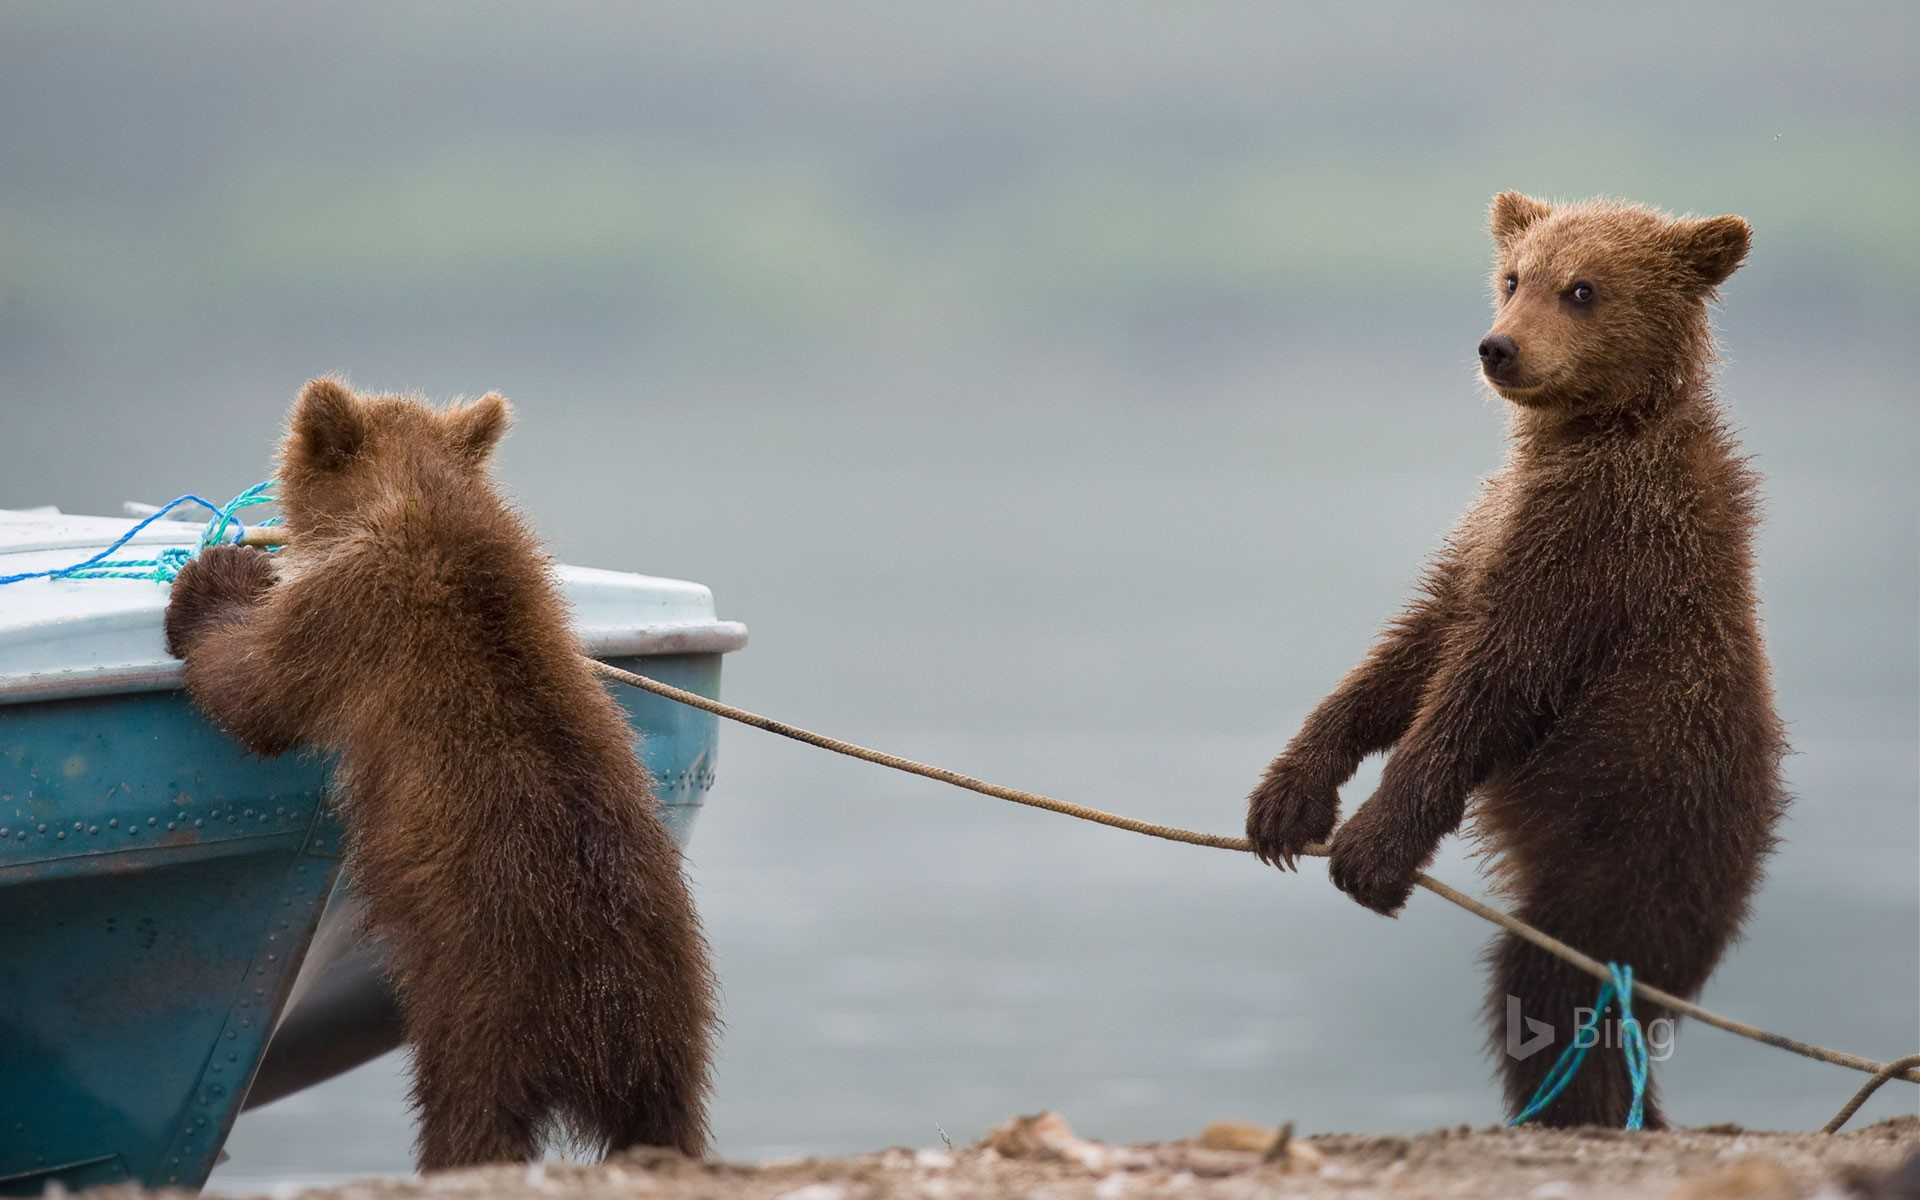
\includegraphics[width=\textwidth]{images/BingWallpaper-2019-04-01.jpg}
	\caption{\imageortable\bfseries 第一张图}
    \label{Wallpaper}
\end{figure}


\begin{table}
    \centering\imageortable
    \renewcommand{\arraystretch}{1.5}
    \caption{\imageortable\bfseries 测试}
    \begin{tabular}{>{\centering\arraybackslash}p{1.5cm}>{\centering\arraybackslash}p{1.5cm}>{\centering\arraybackslash}p{1.5cm}>{\centering\arraybackslash}p{1.5cm}}\hline
        标题1 & 标题2 & 标题3 & 标题4\\ \hline
        111 & 一个测试 & $a$ & $a+b$\\
        222 &  &  & \\
        333 &  &  & \\ \hline 
    \end{tabular}
    \label{tab:my_label}
\end{table}

参考文献\upcite{何祚镛2007近场声全息技术应用有关物理问题研究}的引用。

\subsection{国内外研究现状}
\begin{equation}
    y(x)=y_0+\int_{x_0}^xf(t,y(t))\text{d}t
\end{equation}
\subsubsection{研究方向及进展}
	
\subsubsection{存在问题}
	
\subsection{研究展望}

\bibliographystyle{gbt7714-numerical}
\phantomsection		% 要想目录中参考文献的超链接正确需要加这一语句
\subsection{参考文献}
{\normalfont\CJKfamily{Songti}\zihao{5}\setlength{\baselineskip}{14pt}
\renewcommand{\refname}{\vspace{-\baselineskip}}
\bibliography{reference/refs}}